%%  **********************************************
%
%   The lines beginning with "%" are comments. 
%   Theses comments explain how to use this template for
%   preparing the MCA Fifth Semester Mini-Project Report. 
%
%   The first non-comment line below contains 
%   the matter that go into the preamble of 
%   the input file. These are collected in a 
%   file named "preamble.tex". 
%
%   Do not make any changes in the first 
%   non-comment line below.
%
%%
\documentclass[11pt, oneside, a4paper]{book}
\usepackage[T1]{fontenc}
\usepackage{graphicx, fancyhdr, amsmath, times, enumerate, amssymb, calc, multirow, setspace, array, url}
\usepackage[a4paper,width=150mm,top=35mm,bottom=35mm,bindingoffset=6mm]{geometry}
%% Reference: https://www.overleaf.com/learn/latex/
%% How_to_Write_a_Thesis_in_LaTeX_(Part_2):_Page_Layout
%%
\newcommand{\VAtitle}[1]%
{\def\vtitle{#1}}%
\newcommand{\VAauthora}[1]%
{\def\vauthora{#1}}%
\newcommand{\VAauthorb}[1]%
{\def\vauthorb{#1}}%
\newcommand{\VAauthorc}[1]%
{\def\vauthorc{#1}}%
\newcommand{\VAadmissionyear}[1]%
{\def\vadmissionyear{#1}}%
\newcommand{\VAregisternumbera}[1]%
{\def\vregisternumbera{#1}}%
\newcommand{\VAregisternumberb}[1]%
{\def\vregisternumberb{#1}}%
\newcommand{\VAregisternumberc}[1]%
{\def\vregisternumberc{#1}}%
\newcommand{\VAguide}[1]%
{\def\vguide{#1}}%
\newcommand{\VAhod}[1]%
{\def\vhod{#1}}%
\newcommand{\VAdept}[1]%
{\def\vdept{#1}}%
\newcommand{\VAclass}[1]%
{\def\vclass{#1}}%
\newcommand{\VApaper}[1]%
{\def\vpaper{#1}}%
%%
\linespread{1.3}
\setcounter{secnumdepth}{4}
%%
%
%   No changes in the next non-comment line.
%
\begin{document}
%
%***************************************************
%
%   No changes in the next comment line.
%
\VApaper{20MCA245 Mini Project}%
%
%   In the next line, replace "Report Title" by 
%   the title of your project/thesis.
%
\VAtitle{HireEngine: AI Recruitment Agent}%
%
%   In the next line, replace "Student1" 
%   by name of first student. 
%   Write full name without, repeat without, Mr or Ms
%
\VAauthora{Mahmood Ahsan K}%
%
%

%   In the next line, replace "RegNo1" by the
%   University Examination Register Number of first student.
%
\VAregisternumbera{VAS25MCA-2040}% 
%
%   In the next line, replace "RegNo2" by the 
%   University Examination Register Number of second student.

%
%   In the next line, replace "2024" by the year of  
%   your admission to the College.
%
\VAadmissionyear{2025}
%
%   In the next line, replace "Guide" by 
%   the full name of your guide or supervisor 
%   with Mr. or Ms. or Dr. or Prof.
%
\VAguide{Mr. Manesh D}% 
%
%   No changes in the next three non-comment lines.
%
\VAhod{Dr. Reji C Joy}
%
\VAdept{Computer Applications}%
%
\VAclass{S3 MCA}%
%
%   The next line is code to print the first few pages: 
%       1. Title page
%       2. Bona Fide Certificate from MCA Dept
%       3. Declaration
%       4. Acknowledgment
%   No changes in the next non-comment line.
%
%
%   Redefining plain page style
%  
\fancypagestyle{plain}{%
\fancyhf{} % clear all header and footer fields
\fancyhead[L]{{\small \vtitle}}
\fancyhead[R]{\bf \thepage}
\fancyfoot[C]{\bfseries \thepage} 
\fancyfoot[L]%
{{\scriptsize Department of \vdept, 
Vidya Academy of Science \& Technology, Thrissur}}
\fancyfoot[R]%
{
\includegraphics[width=0.75cm]{VidyaLogo}}%
\fancyfoot[C]{ }%
\renewcommand{\headrulewidth}{1pt}%
\renewcommand{\footrulewidth}{0.5pt}%
}%
%
\pagestyle{empty}
%
%%
\pagenumbering{roman}
\thispagestyle{empty}
%%
\quad
\begin{center}

\sffamily\small
%
\begin{spacing}{2}
{\fontsize{15.5}{20}\selectfont \bfseries \MakeUppercase{\vtitle}}\\[5cm]
\end{spacing}
%

\begin{spacing}{1.25}
A Mini Project Report submitted by\\[0.25cm]
{\bfseries \vauthora}

{(\vregisternumbera)}\\[0.1mm]


\quad\\[0.25cm]
to APJ Abdul Kalam Technological University\\
in partial fulfillment of the requirements for the award of the degree of\\
Master of Computer Applications
\end{spacing}
%
\quad\\[5cm]
%   Logo
%
\includegraphics[width=0.12\textwidth]%
{VidyaLogo}\\[0.3cm]
%
%   Department particulars
%
\begin{spacing}{1.25}
{\normalsize \sffamily \bfseries Department of \vdept}\\
{\small \sffamily Vidya Academy of Science \& Technology\\ 
\small Thalakkottukara, Thrissur - 680 501}\\
{\sffamily October 2026}
\end{spacing}
%%
\end{center}
%%
%\newpage
%%

%
\clearpage
%
\addcontentsline{toc}{chapter}{Certificate from College}
%
%\vspace*{\fill}
\quad\\[0.25cm]
\pagestyle{plain}
\begin{center}
%
%
%   Department particulars
%
{\Large \bf Department of Computer Applications \par  }%\\[0.2cm]
{\large \bf Vidya Academy of Science \& Technology\par}%\\
{\normalsize \bf Thalakkottukara, Thrissur - 680 501\\
({\tt http://www.vidyaacademy.ac.in})\par}
\qquad\\[0.5cm]
%
%   Logo
%

\includegraphics{VidyaLogo}\\[0.75cm]
%
{\Large \bf CERTIFICATE}\\[0.75cm]
%
\end{center}
%
%   Certificate statement
%
This is to certify that the report titled 
{\bf \vtitle} is a bona-fide record of the 
work related to the paper \vpaper\  done  by 

\begin{center}
{\bf \vauthora\  
(Reg. No. \vregisternumbera) } \\ 

\end{center}
   of  \vclass\  
(\vadmissionyear\ admissions) class 
of Vidya Academy of Science \& Technology, 
Thrissur - 680501 in partial fulfillment of the 
requirement for the award of the Degree of Master of \mbox{Computer} Applications  of APJ Abdul Kalam Technological University. \\
%
%   Spaces for signatures 
%
\begin{center}
\begin{tabular}{p{0.10\textwidth}p{0.35\textwidth}p{0.10\textwidth}p{0.35\textwidth}}
%
\multicolumn{2}{l}{\bf Guide/Supervisor}    
&\multicolumn{2}{l}{\bf Head of Department}   \\
%
Name & : \vguide    & Name & : \vhod \\
%
Signature&: ...........................................
\qquad\quad   & 
Signature&: ...........................................\\
%
Date &: \today    & Date &: \today \\
%
\end{tabular}
\\[0.75cm]
%
%   Space for seal of Department
%
{\small (Seal of Department of \vdept)}
\end{center} 
%
\vspace*{\fill}
%
%   End of Certificate
%  
\clearpage
%
\addcontentsline{toc}{chapter}{Declaration by Student}
\thispagestyle{empty}
\chapter*{Declaration}
%
I, {\bf \vauthora} , studying in Third Semester MCA (2025 admissions) class of Vidya Academy of Science \&\  Technology, Thrissur -- 680501,    hereby declare that the project report 
(``\vtitle'') submitted by me  is a bona fide work done by me
under supervision of \vguide. This submission represents my ideas in
my own words and where ideas or words of others have been included, I have adequately
and accurately cited and referenced the original sources. I also declare that I have
adhered to ethics of academic honesty and integrity and have not misrepresented or
fabricated any data or idea or fact or source in my submission. I understand that any
violation of the above will be a cause for disciplinary action by the institute and/or the
University and can also evoke penal action from the sources which have thus not been
properly cited or from whom proper permission has not been obtained. This report has
not been previously formed the basis for the award of any degree, diploma or similar title
of any other University. 

\qquad\\[1cm]
\begin{tabular}{p{0.05\textwidth}p{0.27\textwidth}p{0.01\textwidth}p{0.21\textwidth}p{0.35\textwidth}}
%
Place &: Thrissur -- 680501\qquad      &  &Signature of student  &: ......................................\\
Date  &: \today                        &   &Name of student       &: \vauthora \\
     
\end{tabular}
\clearpage
%
\addcontentsline{toc}{chapter}{Acknowledgment}
%
\chapter*{Acknowledgment}
%
\index{acknowledgment}
I wish to record my indebtedness and thankfulness 
to all who helped me prepare this Report\index{seminar report} titled 
`` \vtitle\ ''  and present it in a satisfactory way. This Report is part of my work related to the paper \vpaper.

I am especially thankful to my
guide and supervisor \vguide\  in the Department of \vdept\  
for giving me valuable suggestions and 
critical inputs in the preparation of this report. 
I am also thankful to \vhod, 
the Head of \vdept\  Department
for encouragement. 

My friends in my class have always been 
helpful and I am grateful to them for 
patiently listening to my presentations on my work related to the Project. 

\begin{flushright}
\vauthora\\ {\footnotesize (Reg. No. \vregisternumbera)}\\
\vclass\  (\vadmissionyear\  Admissions)\\
Vidya Academy of Science \& Technology\\
Thrissur -680 501.
\end{flushright}
%
\clearpage
%
%
%****************************************************
%
%   No changes in the next two non-comment lines. These
%   lines are intended to create the Synopsis page and 
%   to add the the item "Synopsis" to 
%   table of contents.
%
\chapter*{Synopsis}
\addcontentsline{toc}{chapter}{Synopsis}
%
%   Enter below a synopsis of the project report. 
%   The two lines given
%   are to be deleted before entering actual abstract.

HireEngine is a web-based recruitment platform that organizes job postings, candidate applications, resume review, and interview rounds in a single workflow. Recruiters create a job, define required skills and interview availability, and share a public application link. Candidates submit their details and a PDF or DOCX resume through that link.

The first round processes the resume by extracting its text, removing contact details, applying AI-assisted anonymization, and producing a rubric-based score for recruiter review. Candidates selected by the recruiter can proceed to a timed AI voice interview. The interview transcript is evaluated against role-related criteria and shown as advisory information. Candidates who advance to the final round attend a scheduled video interview, where the recruiter records feedback and a selection decision. Automated email tasks and scheduled background work support the process, including cleanup of candidate application data after the configured 90-day retention period.

The application uses Django and Django REST Framework for its API, PostgreSQL for persistent data, Celery and Redis for background processing, and React for the browser interface. OpenAI services support resume processing and realtime voice interviews, while LiveKit provides video interview rooms. AI scores assist review; recruiters retain responsibility for advancement and final hiring decisions.
%
%***************************************************
%
%   The next three lines creates a Table of Contents 
%   in a new page. 
%   Do not delete this. There must be a Table of Contents.
%
\clearpage
\addcontentsline{toc}{chapter}{Table of Contents}
\tableofcontents
%
%   The next three lines create a page containing a 
%   List of Tables. Delete them if there are no 
%   tables in your project report. 
%
\clearpage
\addcontentsline{toc}{chapter}{List of Tables}
\listoftables
%
%   The next three line create a page containing a 
%   List of Figures. Delete them if there are no 
%   figures in your project report.
%
\clearpage
\addcontentsline{toc}{chapter}{List of Figures}
\listoffigures
%
%***************************************************
%
\mainmatter
%
\clearpage
\quad\vfill
\begin{center}
{\Huge \bf PROJECT REPORT}
\end{center}
\vfill
\clearpage
%
%
%   The main contents of the paper begin here. 
% 
%
%   *********************  CHAPTER ***********************
%
%  
\chapter{INTRODUCTION}

%
\section{Problem Definition}
Recruitment information is often split among job boards, email, and spreadsheets. This fragmentation makes it harder to track applicants, compare qualifications consistently, coordinate interviews, and apply data-retention rules. Manual resume review can expose personal details before job-related qualifications are considered. HireEngine brings these tasks into one workflow and supports anonymized, rubric-based evaluations; recruiters retain responsibility for advancement and hiring decisions.
%
\section{Objectives}
The objectives are to provide secure recruiter accounts and job management; accept applications with consent and resumes; redact and score resume text; support CV review, AI voice, and HR video rounds; coordinate interviews; record feedback and outcomes; send notifications; and apply the candidate-data retention policy.
%
\section{Purpose of the Project}
The project gives recruiters one application for managing hiring from job creation to the final decision. Candidates apply and attend interviews through browser pages; recruiters review applications, control advancement, and record feedback. AI assists with resume and interview evaluation, while hiring decisions remain with the recruiter.

%
%   *********************  CHAPTER ***********************
%
%
\chapter{SYSTEM ANALYSIS}
%
\section{The Existing System}	
In a conventional hiring process, job details, resumes, interview schedules, and feedback may be maintained in separate documents or services. Recruiters must manually update candidate status and coordinate available times, making the process difficult to audit and potentially inconsistent. Separate tools can also lead to repeated data entry, missed communications, and uncertainty about the status of a candidate. A centralized system can reduce this administrative fragmentation and make progress visible to the recruiter.

%< Describe your various components here >
\section{Proposed System}
HireEngine provides a recruiter workspace and public candidate pages connected to a Django API. The system follows three rounds. In Round 1, a candidate submits an application and resume through a job-specific link. A background task extracts text from supported PDF or DOCX files, removes contact details, performs AI-assisted anonymization, and creates a rubric-based CV score. The recruiter reviews the applications and chooses which candidates to advance.

In Round 2, shortlisted candidates receive an invitation to a scheduled AI voice interview. A time-limited OpenAI Realtime session conducts a role-focused interview. The transcript is scored against technical, depth, communication, and relevance criteria and is made available to the recruiter as advisory information. In Round 3, selected candidates attend a LiveKit video interview with the recruiter. The recruiter records a rating, notes, and a selected or rejected decision. Email notifications, deadline checks, interview scheduling, and retention cleanup are supported by background tasks.
%
%
%   *********************  CHAPTER ***********************
%
%
\chapter{FEASIBILITY STUDY}
%
\section{Technical Feasibility}
HireEngine uses Python 3.12, Django 5.1, Django REST Framework, PostgreSQL 16, Celery 5, Redis 7, React 19, Vite, and Docker Compose. Its main services can be run with the provided container configuration. OpenAI, LiveKit, and SMTP credentials are needed for their corresponding external features. Camera and microphone access requires HTTPS or a browser localhost secure context.
%
\section{Economical Feasibility}
The backend, frontend, database, queue, and container technologies are available as open-source software. Production costs may include hosting, storage, email, OpenAI API usage, and LiveKit usage. Actual expenses depend on applicant and interview volumes and the selected service plans, so they should be estimated for the intended deployment.
%
\section{Operational Feasibility}
Recruiters use the dashboard to create jobs, review candidates, schedule interviews, and record decisions. Candidates apply and join interviews through public or private links. Users need a current browser and network access; interview rounds require microphone or camera permissions. AI evaluations are advisory, and recruiters retain control of advancement and hiring decisions.
%
\chapter{SYSTEM DESIGN}
%
\section{Input Design}
The application accepts the following inputs through browser forms and API endpoints.
\begin{itemize}
\item \textbf{Recruiter registration:} full name, company name, work email, password, and optional company description, address, and timezone.
\item \textbf{Job details:} job title, description, required skills, minimum experience, employment type, location, work mode, optional salary range, application deadline, and shortlist limits.
\item \textbf{Candidate application:} full name, email, phone number, consent, and a resume in PDF or DOCX format.
\item \textbf{Interview availability:} interview round and start and end times for the available scheduling window.
\item \textbf{Recruiter evaluation:} advancement choice, interview feedback, rating, notes, and final decision.
\end{itemize}
%
\section{Output Design}
The application displays recruiter dashboard statistics, job stages, applications, CV-processing status, scores and score breakdowns, interview schedules, transcripts, feedback, and final decisions. Candidates receive application confirmation and round-invitation messages and can view the relevant application or interview information through public links. Error responses communicate invalid forms, duplicate applications, expired deadlines, or unavailable interview windows.
%
\section{Database Design}
HireEngine uses PostgreSQL. Recruiter accounts are represented by the custom User model. A recruiter may own multiple Job records. Each job may have applications, round records, and availability windows. An Application belongs to one job and stores candidate contact information, resume location, anonymized text, processing status, CV score, and pipeline status. An Interview is linked to a job, an application, and the responsible recruiter; an AIResult or Feedback record stores the relevant evaluation. EmailLog records notification delivery status.

The data model uses UUID primary keys for the principal records. Normalized email and phone numbers are unique per job, each job has a unique public form slug, and only one interview of each kind can be created per application. Database constraints validate shortlist sizes and timing values and prevent overlapping reservations for the same recruiter and interview kind. The PostgreSQL exclusion constraint uses the btree\_gist extension.

Deleting a job cascades to its applications and related interview records. Candidate application data and associated resume files are removed by the scheduled cleanup task after the configured 90-day retention period for completed or removed jobs. Recruiter and candidate access is separated between authenticated recruiter endpoints and public application or token-based interview endpoints.
%
%
%   *********************  CHAPTER ***********************
%
%
\chapter{IMPLEMENTATION, TESTING AND VALIDATION}
%
\section{Implementation}
The backend is divided into Django applications for accounts, jobs, applications, interviews, notifications, and AI services. The React client communicates with the API through HTTP requests. Recruiter endpoints use JWT authentication; candidate application and interview endpoints are selectively public and use job slugs or interview tokens.

When a candidate submits a resume, the application is stored and asynchronous Celery tasks process the file and send a confirmation email. Text extraction supports PDF and DOCX documents and rejects unsupported or insufficiently text-based input. Contact details and URLs are removed before the anonymization and scoring steps. CV scoring uses skills, experience, and education categories with a total score out of 100. When OpenAI is unconfigured or unavailable, deterministic fallback routines are available for anonymization and scoring.

The AI interview service builds instructions from the job details and interview prompt and requests a short-lived OpenAI Realtime session credential. Once completed, the transcript is scored and stored with score details. The HR interview flow creates a LiveKit room token and allows the recruiter to record feedback. Celery workers perform resume and email tasks, while Celery Beat schedules recurring deadline and retention jobs. Environment variables are used for service configuration and credentials.
%
\section{Testing Methods}
The source repository includes Django tests for the main backend applications. The account tests cover email verification, OTP expiry, lockout after invalid attempts, resend cooldown, and login. Job tests cover deadlines, ranking, shortlist capacity, invitations, and round transitions. Application tests cover public application submission, consent, supported resume formats, duplicate prevention, anonymization, and retention cleanup. Interview tests cover interview state and timing, AI results, video-room access, and recruiter feedback. Notification tests cover email task behavior.

The application tests use Django's test framework and the REST framework API client to exercise both successful and rejected requests. They check consent, resume formats and extracted text, duplicate contact details, and persisted application status, so the expected API behavior and stored data are both considered.

These test cases are present in the repository; this report does not claim a particular full-suite pass result.
% < Describe the various Testing methods used here >
\section{Validation}
Input validation is applied at the API serializer and model levels. Resume handling validates file type, readability, and minimum extracted text length. Database constraints protect unique application identifiers and interview scheduling rules. Authenticated recruiter views restrict job and application access to the owning recruiter, while public candidate actions use a job slug or interview token. Interview scores are constrained to their configured rubric ranges and are presented as advisory outputs. Recruiters make the final decisions.
%	< Validation done in the project >
%
%   *********************  CHAPTER ***********************
%
\chapter{CONCLUSION}
HireEngine centralizes job setup, application intake, resume processing, interview scheduling, recruiter feedback, and candidate outcome tracking. Its three-round workflow reduces fragmented administration by bringing application review, interview coordination, notifications, and decisions into one platform. PostgreSQL constraints help preserve data integrity, while Celery and Redis handle time-consuming background tasks and scheduled work.

The platform combines automated resume processing and AI-assisted interviews with recruiter review. The resulting scores are advisory: recruiters decide whom to advance and make the final hiring decision. The implemented data model, interview workflow, and retention task provide a foundation for a complete hiring process. Before production use, the external email, AI, video, storage, and database services require suitable configuration, monitoring, and operational controls.

The project demonstrates how these components can be combined while keeping recruiter decisions central. Its modular backend and browser-based interfaces provide a base for further evaluation with recruiters and candidates before wider deployment.
%
%   *********************  CHAPTER ***********************
%
\chapter{SCOPE FOR FUTURE ENHANCEMENT}
The project can be extended in several ways.
\begin{itemize}
\item \textbf{Audit trail:} record recruiter stage changes and decisions.
\item \textbf{Score explanations:} show clearer evidence for CV and interview rubric scores.
\item \textbf{Fairness evaluation:} assess anonymization and scoring with a consented, representative dataset.
\item \textbf{Accessibility and localization:} add configurable rubrics, accessible candidate experiences, and additional languages.
\item \textbf{Production operations:} improve deployment automation, secret management, monitoring, backups, and retention controls.
\item \textbf{Expanded testing:} add end-to-end coverage for concurrent scheduling and external-service failures.
\end{itemize}
These improvements would make the hiring process more transparent and reliable as usage grows. They should be prioritized using recruiter and candidate feedback, while considering fairness, accessibility, and data protection requirements.
%
%
%   *********************  CHAPTER ***********************
%
%%%%%%%%%%%%%%%%%%%%%%%%%  APPENDICES %%%%%%%%%%%%%%%%%%%%%
%
\clearpage
\addcontentsline{toc}{chapter}{APPENDICES}
\appendix
\quad\vfill
\begin{center}
{\Huge \bf APPENDICES}
\end{center}
\vfill
\clearpage
%
%
%   *********************  CHAPTER ***********************
%
%
\chapter{SCRUM PROCESS ARTIFACTS}
%
\section{Product Backlog}
%
The work items and effort estimates below are reconstructed from the implemented project features. The estimates are illustrative and are not recorded actual hours.
%
\renewcommand{\arraystretch}{1.25}
\begin{center}
\begin{tabular}{|m{0.08\textwidth}|m{0.15\textwidth}|m{0.5\textwidth}|m{0.1\textwidth}|}
\hline
{\bf Priority} & {\bf Product backlog items} & {\bf User story} & {\bf Estimate (Hours)}\\
\hline
1 & Recruiter accounts & As a recruiter, I want to manage hiring securely. & 24 \\
\hline
2 & Job management & As a recruiter, I want to create and publish jobs for candidates. & 32 \\
\hline
3 & Candidate applications & As a candidate, I want to submit my resume through a job link. & 28\\
\hline
4 & CV review & As a recruiter, I want anonymized resumes and scores for review. & 40\\
\hline
5 & AI voice interviews & As a candidate, I want to complete a scheduled voice interview. & 40 \\
\hline
6 & HR video interviews & As a recruiter, I want to record interview feedback and final decisions. & 40\\
\hline
\end{tabular}
\end{center}
%
\section{Scrum Meeting Details}
The dates below are illustrative sample dates based on the supplied project start month of July 2026. They are not verified meeting records. Dates use day/month format in 2026.
%
\begin{center}
\begin{tabular}{|m{0.03\textwidth}|m{0.05\textwidth}|m{0.3\textwidth}|m{0.2\textwidth}|m{0.2\textwidth}|}
\hline
Sl. No. & Date & Sprint backlog & Product shippable Increment & Important Decisions \\
\hline
1 & 10/7 & Account verification and API foundation & Recruiter registration and login & Use verified email and JWT authentication. \\
\hline
2 & 24/7 & Jobs and candidate applications & Job form and public application flow & Validate consent and resume submissions. \\
\hline
3 & 14/8 & Resume processing and CV review & Extracted, anonymized, scored CVs & Treat automated scores as advisory. \\
\hline
4 & 4/9 & AI voice interview & Realtime interview and transcript scoring & Restrict interview to role-related questions. \\
\hline
5 & 25/9 & HR video interviews and notifications & Scheduled LiveKit meetings and feedback & Prevent conflicting recruiter interview slots. \\
\hline
6 & 9/10 & Testing and retention tasks & Test coverage and scheduled cleanup & Retain candidate data for the configured 90 days. \\
\hline
\end{tabular}
\end{center}

\renewcommand{\arraystretch}{1}
%
%   *********************  APPENDIX ***********************
%
\chapter{UML DIAGRAMS}
\section{Class Diagram}
%
\begin{figure}[!b]
   \centering
    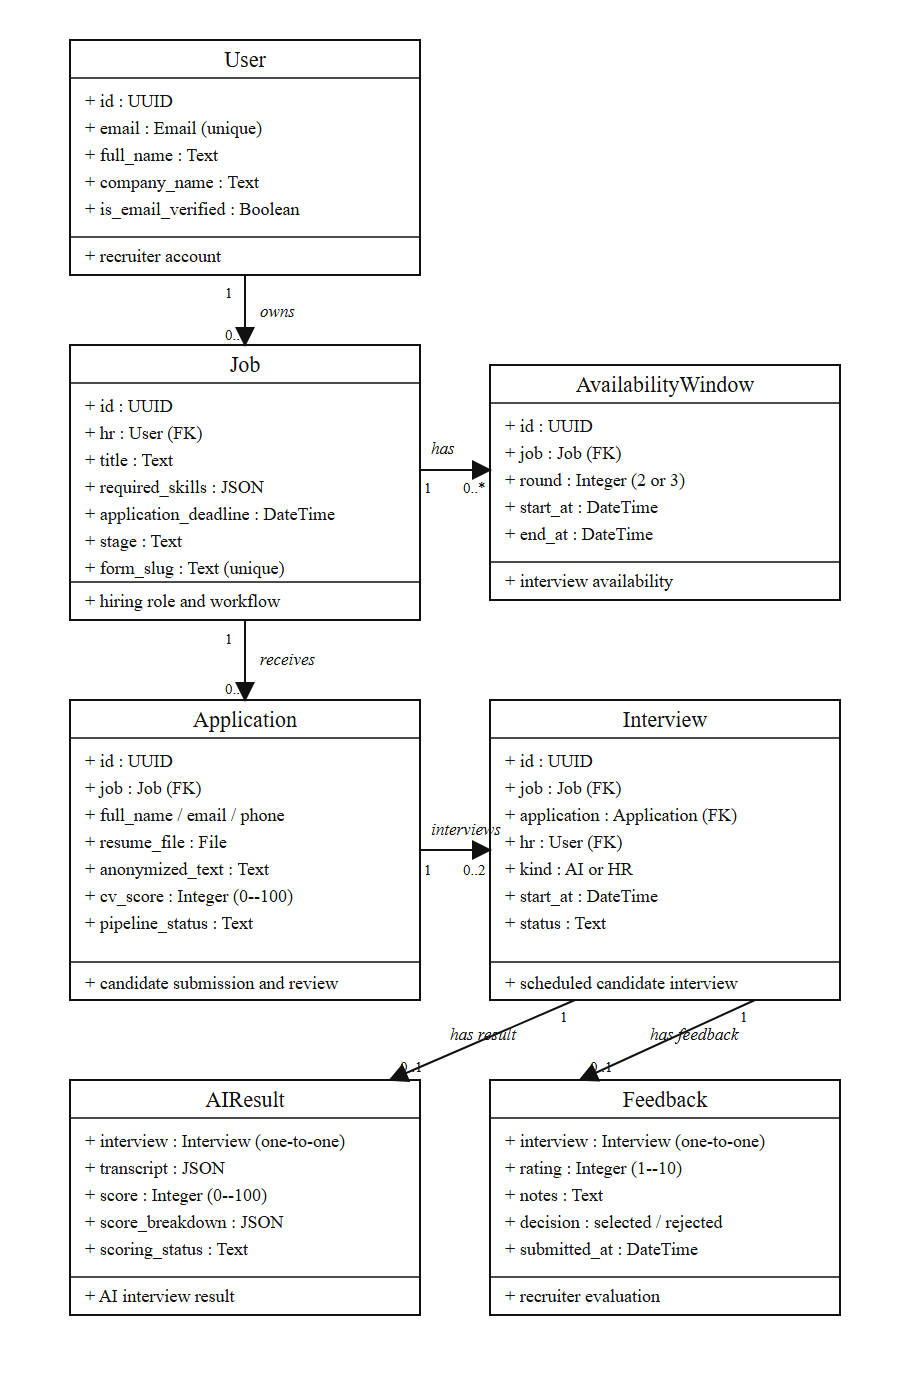
\includegraphics[width=0.5\linewidth,height=0.72\textheight,keepaspectratio]{Class_Diagram.png}
    \caption{Class Diagram of HireEngine}
    \label{fig:class-diagram}
\end{figure}
\section{State Diagram}
\begin{figure}[!b]
   \centering
    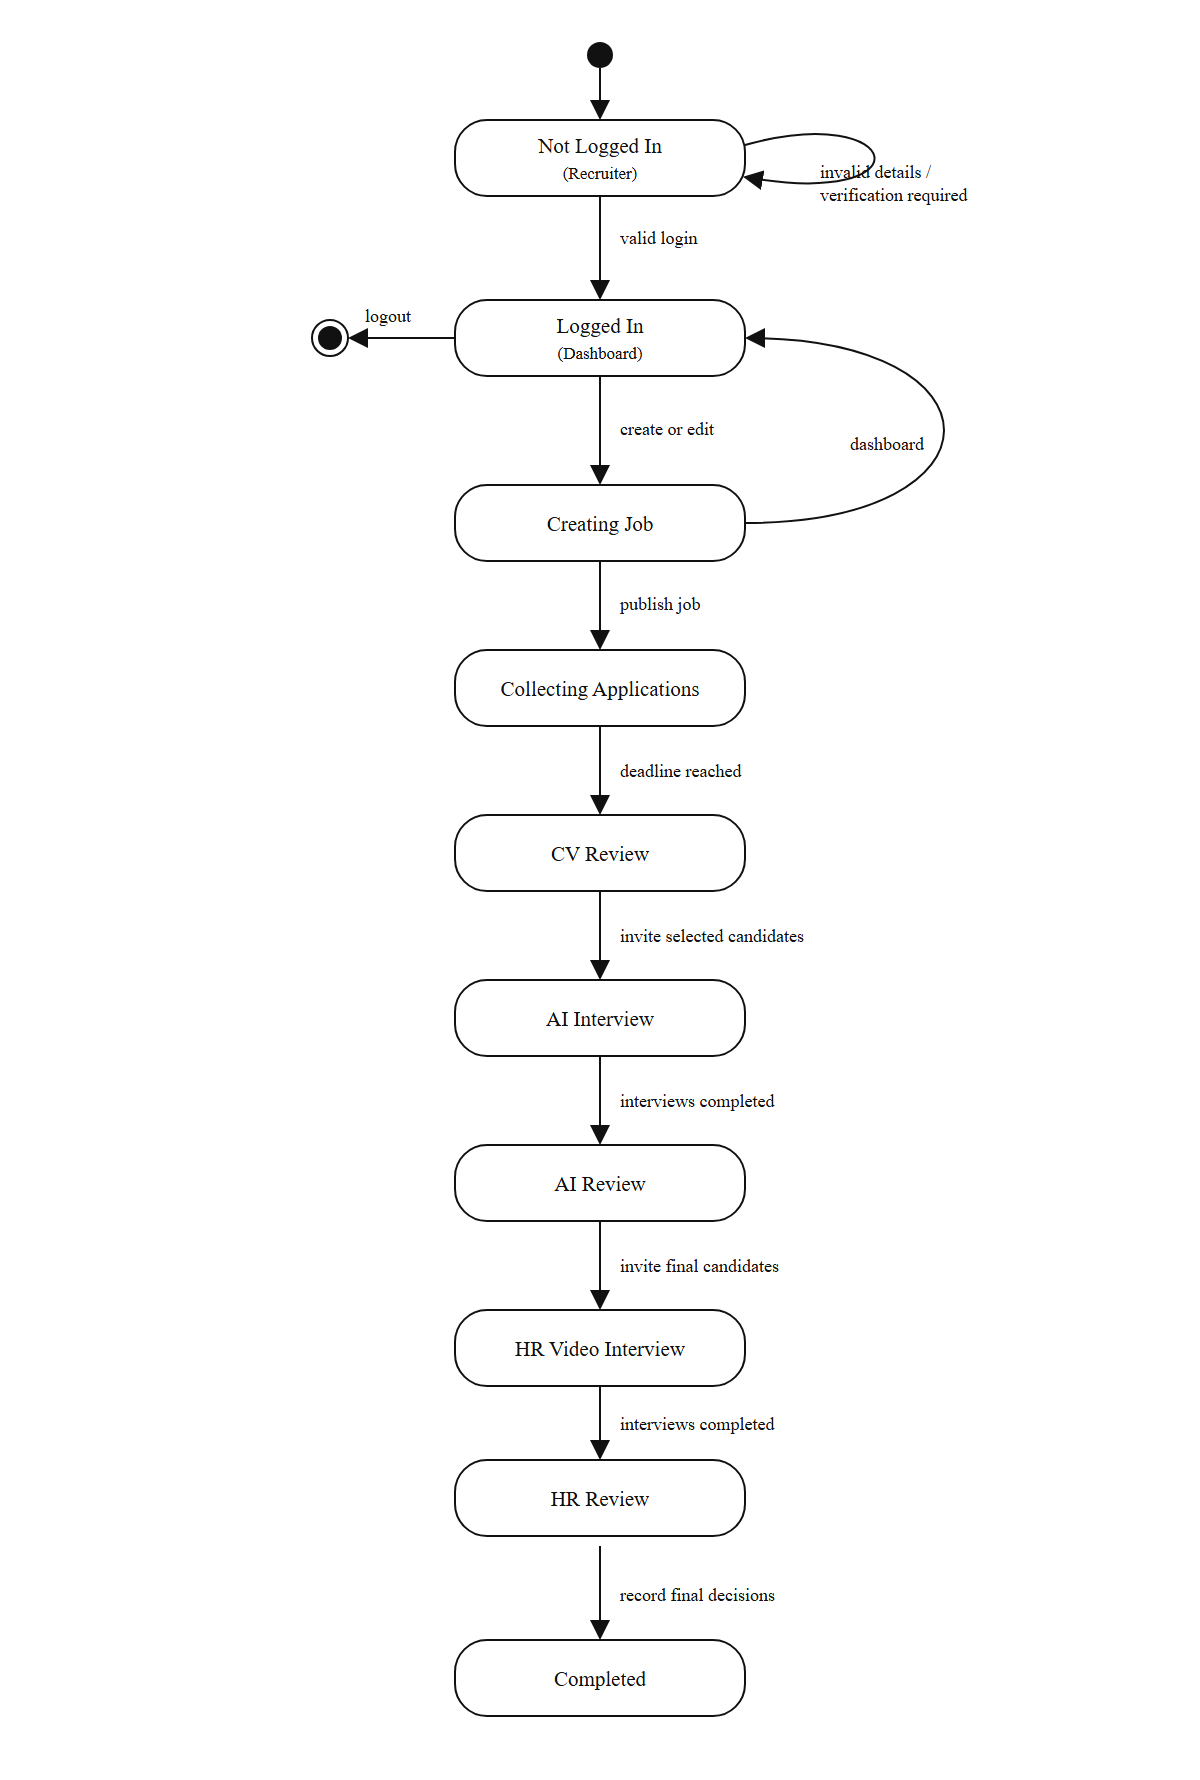
\includegraphics[width=0.5\linewidth,height=0.72\textheight,keepaspectratio]{State_Diagram.png}
    \caption{State Diagram of HireEngine}
    \label{fig:state-diagram}
\end{figure}
%
%
%   *********************  APPENDIX ***********************
%
\chapter{TABLE STRUCTURE}
\begin{table}
 \centering
  \begin{tabular}{|l|l|l|l|l|}
    \hline 
   Sl. No.&  Field&  Datatype&  Constraint& Description \\
     \hline  
    1 & id & UUID &Primary Key  & Recruiter ID\\ 
      \hline 
     2 & email  & Email & Unique & Recruiter login\\
     \hline 
     3  & company\_name & Text & Not Null & Recruiter company \\ 
     \hline
     4 & is\_email\_verified & Boolean & Default false & Email verification status \\
				\hline
    \end{tabular}
    \caption{User table}
\label{table:users}
\end{table}
\begin{table}
 \centering
  \begin{tabular}{|l|l|l|l|l|}
    \hline 
   Sl. No.&  Field&  Datatype&  Constraint& Description \\
     \hline  
    1 & id & UUID &Primary Key  & Job ID\\ 
      \hline 
     2 & hr\_id  & UUID & Foreign Key & Job owner\\
     \hline 
     3  & title & Text & Not Null & Job title \\ 
     \hline
     4 & required\_skills & JSON & Not Null & Role skills \\
     \hline
     5 & stage & Text & Not Null & Pipeline stage \\
				\hline
    \end{tabular}
    \caption{Job table}
\label{table:jobs}
\end{table}
\begin{table}
 \centering
  \begin{tabular}{|l|l|l|l|l|}
    \hline 
   Sl. No.&  Field&  Datatype&  Constraint& Description \\
     \hline  
    1 & id & UUID &Primary Key  & Application ID\\ 
      \hline 
     2 & job\_id  & UUID & Foreign Key & Applied job\\
     \hline 
     3  & resume\_file & File & Not Null & Candidate resume \\ 
     \hline
     4 & cv\_score & Small Integer & 0--100 & CV evaluation \\
     \hline
     5 & pipeline\_status & Text & Not Null & Candidate stage \\
				\hline
    \end{tabular}
    \caption{Application table}
\label{table:applications}
\end{table}
\begin{table}
 \centering
  \begin{tabular}{|l|l|l|l|l|}
    \hline 
   Sl. No.&  Field&  Datatype&  Constraint& Description \\
     \hline  
    1 & id & UUID &Primary Key  & Interview ID\\ 
      \hline 
     2 & application\_id  & UUID & Foreign Key & Related application\\
     \hline 
     3  & kind & Text & AI or HR & Interview type \\ 
     \hline
     4 & start\_at & DateTime & Not Null & Scheduled start \\
     \hline
     5 & status & Text & Not Null & Interview state \\
				\hline
    \end{tabular}
    \caption{Interview table}
\label{table:interviews}
\end{table}

%   *********************  APPENDIX ***********************
%
\chapter{SAMPLE SCREENSHOTS}
\begin{figure}[!htbp]
   \centering
    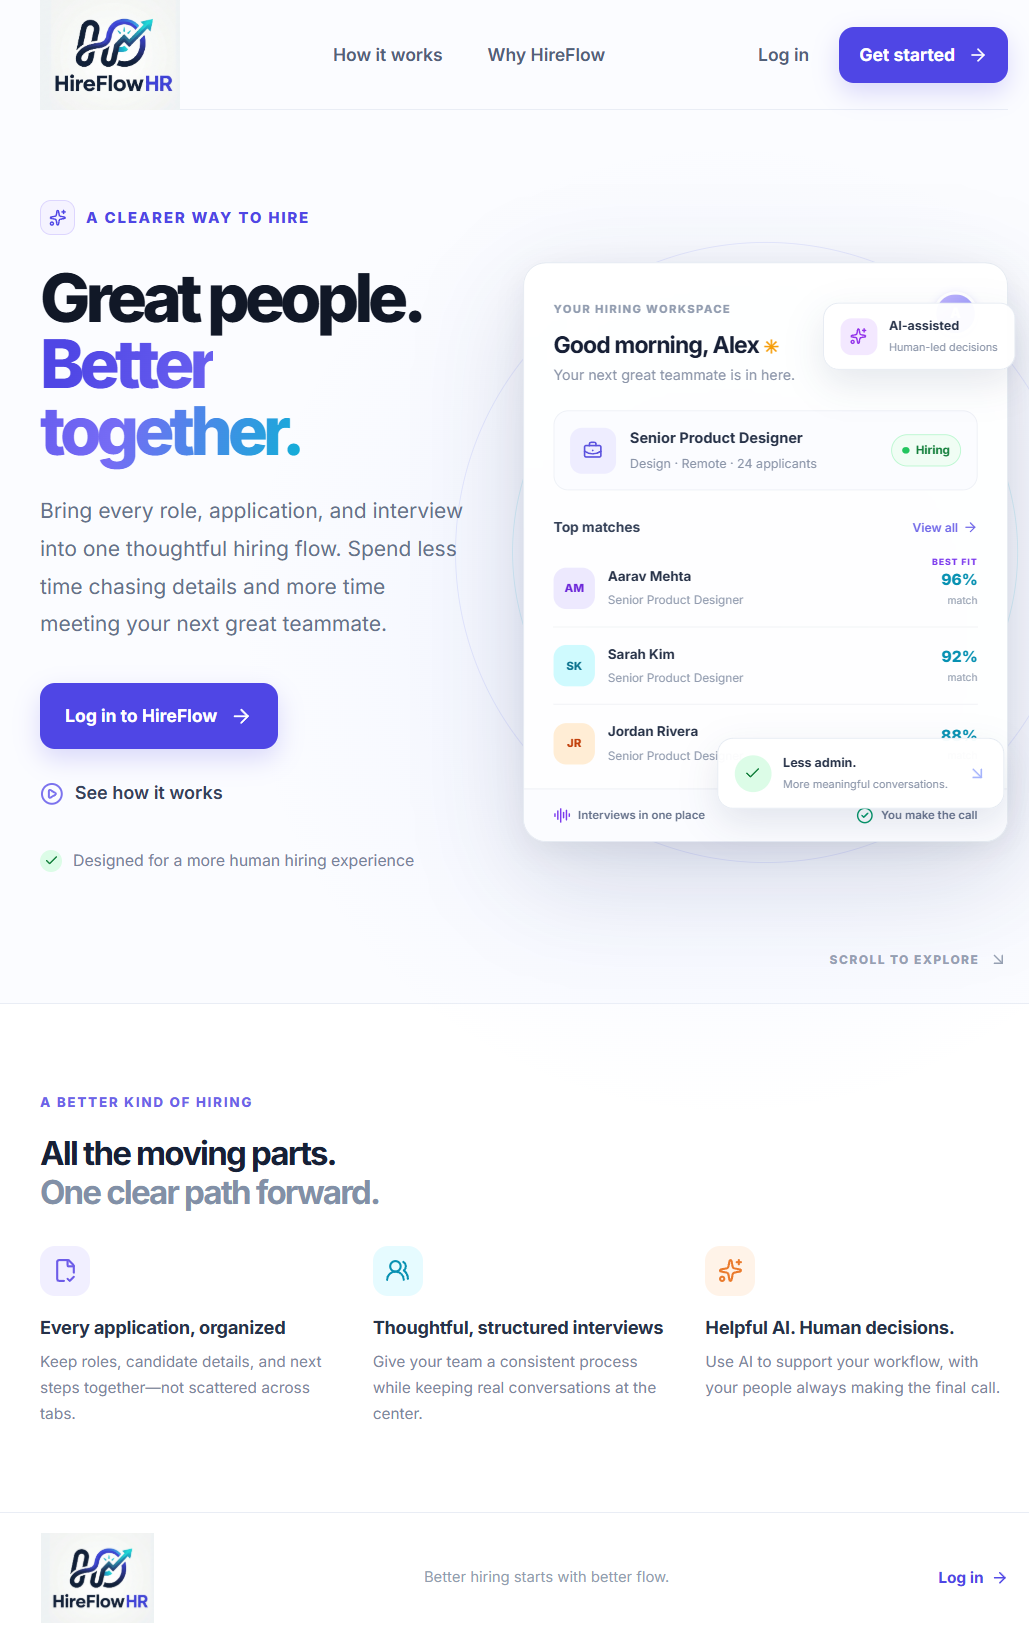
\includegraphics[width=0.5\linewidth]{hireengine-landing.png}
    \caption{Public landing page}
    \label{fig:landing-page}
\end{figure}
\begin{figure}[!htbp]
   \centering
    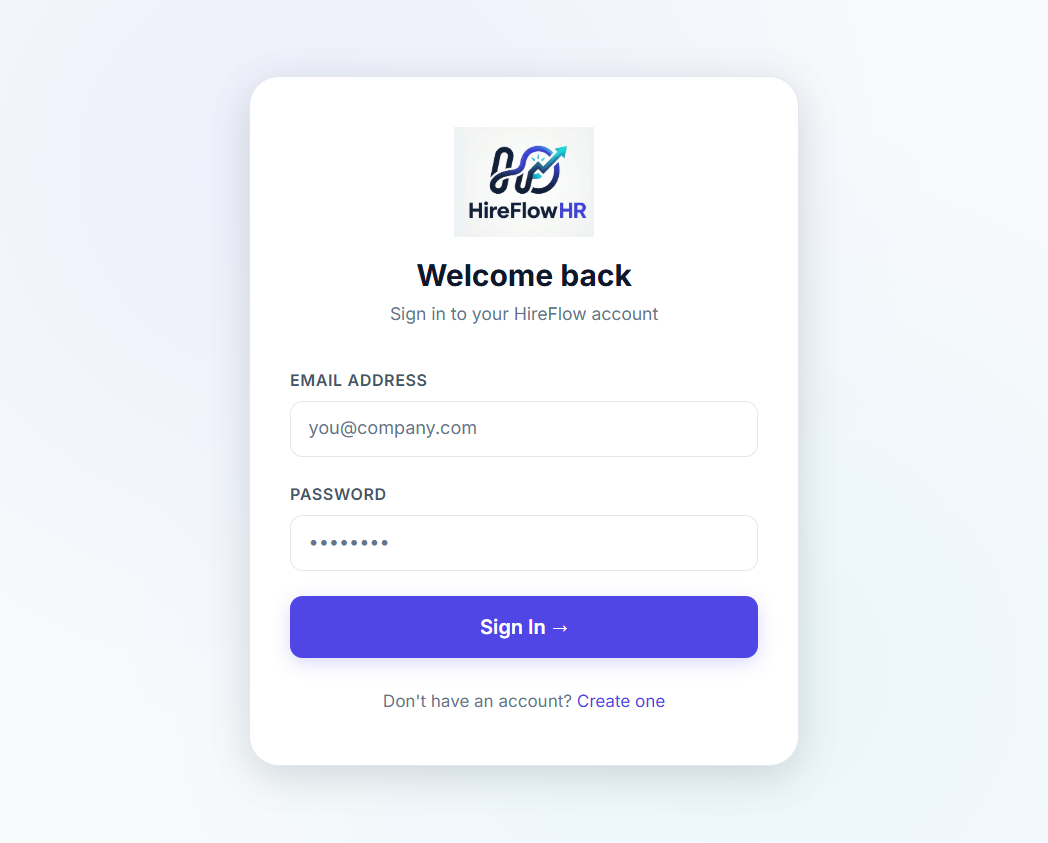
\includegraphics[width=0.5\linewidth]{hireengine-login.png}
    \caption{Recruiter login page}
    \label{fig:login-page}
\end{figure}
\begin{figure}[!htbp]
   \centering
    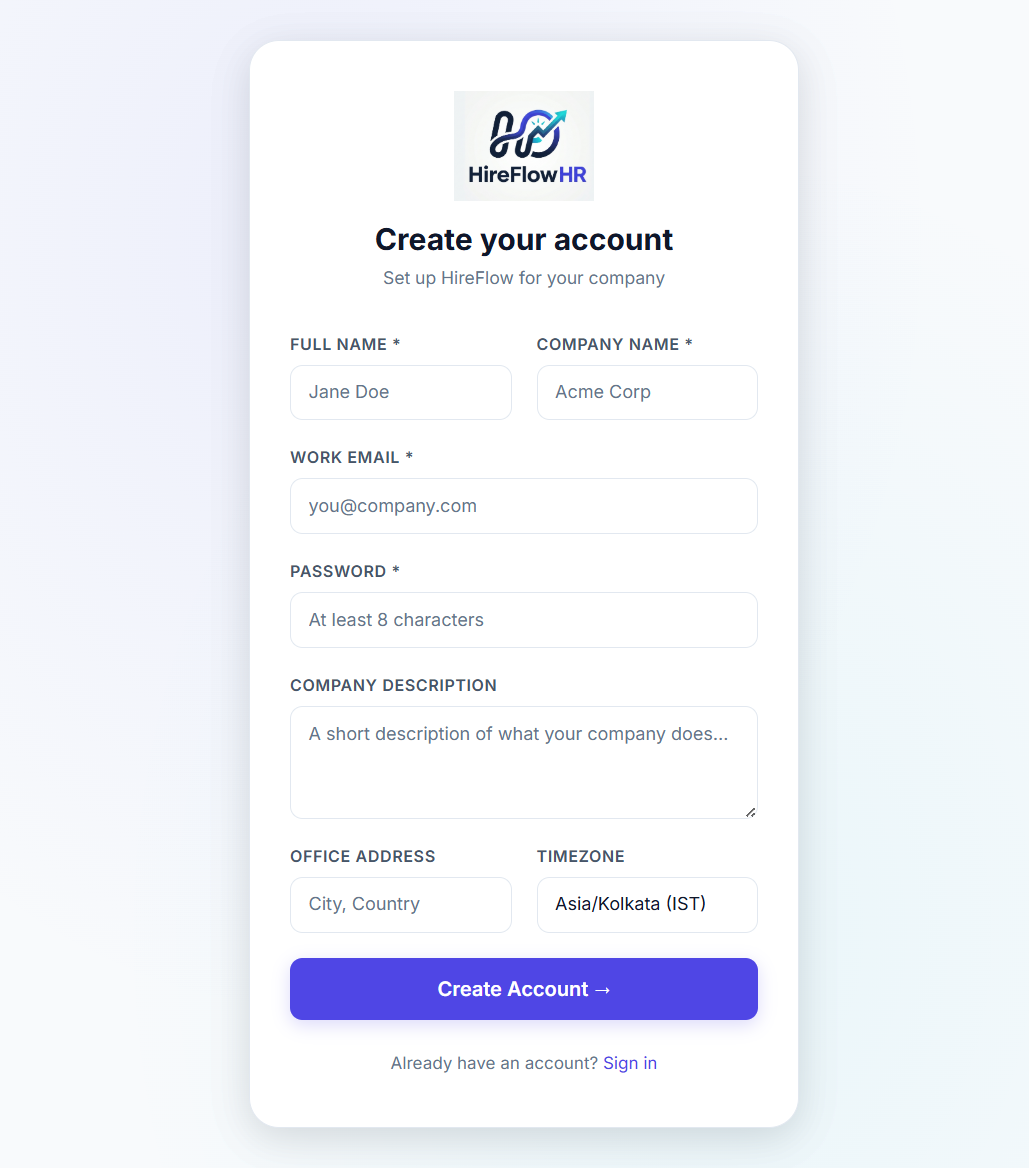
\includegraphics[width=0.5\linewidth]{hireengine-register.png}
    \caption{Recruiter registration page}
    \label{fig:registration-page}
\end{figure}
%
%
% ***   Creating Bibliography   ***
%
% Do not delete the following two lines
%
\clearpage
\addcontentsline{toc}{chapter}{Bibliography}
%
%   The markups for creating the bibliography 
%   begins here. Do not change the two lines 
%   "\begin{thebibliography}{99}" and 
%   "\end{thebibliography}".
%   One sample bibliography item is included. 
%   Each new item is to be preceded by
%   "\bibitem{itemx}".
%   Add additional items if there are any.
%   Bibliography styles:
%   Titles of books   : Italics  {use {\em Title} )
%   URLs of websites  : Type-writer (use {\tt Title} )
%   Titles of papers  : In double quotes (use ``Title")
%
\begin{thebibliography}{99}
%
\bibitem{item1}
Django Software Foundation, {\em Django Documentation}. Available: \url{https://docs.djangoproject.com/}
\bibitem{item2}
Encode OSS Ltd., {\em Django REST framework Documentation}. Available: \url{https://www.django-rest-framework.org/}
\bibitem{item3}
PostgreSQL Global Development Group, {\em PostgreSQL Documentation}. Available: \url{https://www.postgresql.org/docs/}
\bibitem{item4}
Celery Project, {\em Celery Documentation}. Available: \url{https://docs.celeryq.dev/}
\bibitem{item5}
Redis Ltd., {\em Redis Documentation}. Available: \url{https://redis.io/docs/}
\bibitem{item6}
OpenAI, {\em Realtime API Documentation}. Available: \url{https://platform.openai.com/docs/guides/realtime}
\bibitem{item7}
LiveKit, {\em LiveKit Documentation}. Available: \url{https://docs.livekit.io/}
\bibitem{item8}
Meta Platforms, {\em React Documentation}. Available: \url{https://react.dev/}
\bibitem{item9}
Docker, {\em Docker Compose Documentation}. Available: \url{https://docs.docker.com/compose/}
\bibitem{item10}
K. Schwaber and J. Sutherland, {\em The Scrum Guide}, 2020. Available: \url{https://scrumguides.org/}
%
\end{thebibliography}
%
%
%   Printing the last page
%
%
\newpage
\thispagestyle{empty}
\vspace*{\fill}
\begin{flushright}

\includegraphics{VidyaLogo}\\[0.5cm]
{\Large \bf \sf  Department of \vdept\ }\\
{\sf Vidya Academy of Science \& Technology\\
Thalakkottukara, Thrissur - 680 501\\
({\tt http://www.vidyaacademy.ac.in})}
\end{flushright}
%
%
%
%   ***   The end   ***
%
%
\end{document}